\documentclass[10pt,conference]{IEEEtran}
\IEEEoverridecommandlockouts
\usepackage{cite}
\usepackage{amsmath,amssymb,amsfonts}
\usepackage{graphicx}
\usepackage{booktabs}
\usepackage{newtxtext,newtxmath}
\usepackage[hyphens]{url}
\usepackage{microtype}
\usepackage{balance}
\usepackage{listings}
\usepackage{xcolor}
\usepackage{multirow}
\usepackage{enumitem}
\usepackage{algorithm}
\usepackage{algpseudocode}
\usepackage{hyperref}
% IEEE-like lists: hanging indent, modest spacing (avoid leftmargin=*)
\setlist[itemize]{
  leftmargin=1.6em,
  itemindent=0pt,
  labelsep=0.4em,
  itemsep=0.35em,
  parsep=0pt,
  topsep=0.4em,
  partopsep=0pt
}
\setlist[enumerate]{
  leftmargin=1.6em,
  itemindent=0pt,
  labelsep=0.4em,
  itemsep=0.35em,
  parsep=0pt,
  topsep=0.4em,
  partopsep=0pt
}
\lstset{basicstyle=\ttfamily\footnotesize,breaklines=true,frame=single,columns=fullflexible}
% Unnumbered run-in heads (IEEEtran \paragraph becomes a)/b)/c)/...)
\newcommand{\runin}[1]{\medskip\noindent\textbf{#1}\enspace}

\title{Witness-Guided Repair and Dual-Gate Checks\\
for LLM-Generated Guard Specifications}
\author{
\IEEEauthorblockN{Ye Xujun}
\IEEEauthorblockA{East China Normal University\\
Shanghai, China}
% Double-blind: swap to Anonymous Authors / Anonymous Institution.
}

\begin{document}
\maketitle

\begin{abstract}
Large language models synthesise code that often looks correct under everyday
unit tests yet still mishandles thin specification regions---especially
catch-all residuals and ordered overlaps.
Consider a tier classifier whose \texttt{OTHERWISE} branch must return
\texttt{Review}: an LLM candidate can pass every Reject/Pass sample while
silently promoting the mid-band to \texttt{Pass}.
A release dashboard that tracks mean pass rate alone will ship that defect.

We study a bounded \textbf{acceptance check}: release only when every
specification-derived witness matches \emph{and} a structural screen clears
($\mathrm{Accept}\Leftrightarrow\mathrm{Conf}{=}1\wedge\mathrm{Screen}{=}\mathit{pass}$).
HSP-Agile implements this dual-gate check on SOFL/FSF with first-match SMT
witnesses, structured scenario-aware repair feedback, and a configurable
static safety screen.
Here \emph{FAR} is the fraction of faulty mutants that a mode incorrectly
releases; \emph{PDR} is the complementary rejection rate.

When repair still has headroom, scenario-aware feedback improves mean
conformance over test-only feedback by ${+}7.7$\,pp (95\% CI
$[2.3,\,13.6]$); all 14 wins repair catch-all residuals.
On the constructed first-order mutant population, the dual-gate check reduces
FAR from 8.8\% to 5.0\% (PDR 91.2\% to 95.0\%).
At matched budget~$K{=}3$, equal-$K$ Conf.\ places \texttt{M\_eq} at 100.0\%
vs.\ B2 97.5\% (${+}2.5$\,pp; $3/0/117$).
Gemini hard-seed runs support the feedback effect, while GPT-4o/Claude and
public-corpus results reveal frequent saturation.  Test-feedback is therefore
the default; the additional gate is justified when its bounded witness and
mutant criteria match the release context.
\end{abstract}

\begin{IEEEkeywords}
acceptance checking, mutant rejection, specification-guided repair,
ordered guards, LLM synthesis, SOFL, SMT, false accept rate
\end{IEEEkeywords}

%======================================================================
\section{Introduction}
%======================================================================
A release dashboard can look healthy while a residual specification region is
already broken.
LLMs synthesise code that passes busy unit tests yet mishandles catch-all
\texttt{OTHERWISE} bands and ordered overlaps that everyday suites never
sample~\cite{chen2021codex,dakhel2023copilot,zhu1997specification}.
SOFL/FSF makes those regions explicit as first-match
scenarios~\cite{liu1998sofl,liu2004soflbook,li2022qrs_companion}.
We ask whether a team can \emph{refuse} to ship under an acceptance-safety bar
that uses the specification itself as evidence---without full deductive
verification.

\runin{Acceptance criterion.}
Release requires every specification-derived witness to match \emph{and} a
structural screen to clear:
$\mathrm{Accept}\Leftrightarrow\mathrm{Conf}{=}1\wedge\mathrm{Screen}{=}\mathit{pass}$.
We refer to this directly as a \textbf{dual-gate acceptance check}.  It is a
bounded operational criterion over the generated witnesses and configured
screen, not a proof of program safety.
HSP-Agile realises it on SOFL/FSF with SpecIR witnesses, structured
scenario-aware feedback under headroom, and a configurable static screen.
$\mathrm{FAR}$ (False Accept Rate) is the fraction of faulty mutants that a
mode incorrectly releases; $\mathrm{PDR}$ is the complementary rejection rate.

\runin{Primary vignette (catch-all).}
A tier classifier rejects negative scores and passes scores at or above a
floor; everything else falls into \texttt{OTHERWISE} and must return
\texttt{Review}.
An LLM candidate collapses that residual to \texttt{Pass}.
Busy Reject/Pass tests succeed; the mid-band never reaches a human.
Typed IR names the residual scenario (\texttt{others})---the same regime as
all 14 E6 Conf.\ wins over test-only feedback (0/14 ordering repairs).
The intro uses a three-scenario skeleton with residual~$S_3$; BENCH-120 hard
tasks scale the same first-match shape to eight scenarios, so coded wins
refer to residual index~$S_8$.

\runin{Secondary vignette (ordering).}
Ordered tax/sensor overlaps motivate first-match witnesses $\Phi_i$ and
prevention mutants that reorder or drop preemption; they are not the E6 win
set.
A public API ACL reconstruction (\texttt{enforce\_api\_acl}) fail-opens on
\texttt{OTHERWISE} while guest/admin tests pass---Accept stays red.

\runin{Contributions.}
\begin{itemize}
  \item A first-match witness construction that exposes residual and
    precedence regions missed by ordinary test suites.
  \item A controlled comparison showing that scenario-aware repair feedback
    improves mean conformance by ${+}7.7$\,pp over test-only feedback at
    matched $K{=}3$; all 14 wins repair catch-all residuals.
  \item A dual-gate prevention evaluation in which FAR falls from 8.8\% to
    5.0\%, together with cross-model and public-corpus evidence that identifies
    when the additional checking is worth its cost.
\end{itemize}
The evidence therefore separates mechanism (E6), prevention (E2), and
deployment under model or corpus saturation.

%======================================================================
\section{Related Work}
%======================================================================
Closest LLM+verifier systems differ on whether witnesses respect first-match
order, whether repair carries scenario structure, and whether prevention
(PDR/FAR) is measured (Table~\ref{tab:rw}).

\runin{Proof-oriented oracles.}
DafnyBench and Clover target proof
discharge~\cite{loughridge2024dafnybench,sun2024clover}; success is a theorem,
not first-match region coverage.
Our Conf.\ metric is witness agreement under SpecIR, not a proof certificate.
CEGIS-style SMT loops are closer in spirit, but typically synthesise programs
or invariants from logical specs rather than ordered-guard FSF with typed
repair records.

\runin{Verbal and agentic repair.}
Self-Refine, Self-Debug, and Reflexion raise generation success via critique or
verbal memory~\cite{madaan2023selfrefine,chen2024selfdebug,shinn2023reflexion}.
That channel is LLM-as-judge style: useful, but not bound to an executable
first-match oracle---the judge may omit the catch-all scenario index.
CodeT and coding agents optimise repository tasks without an FSF
oracle~\cite{chen2023codet,wang2024opendevin,yang2024sweagent,xia2025agentless,jimenez2024swebench}.
LLM-based APR patches failing tests~\cite{xia2024chatrepair,jiang2023impact,legoues2019apr,bouzenia2024repairagent,fan2023llmrepair};
we evaluate unstructured test feedback as B2 and isolate typed IR in E6.

\runin{Adjacent notations and SOFL.}
Alloy and TLA+ encode structured
constraints~\cite{jackson2002alloy,lamport2002tla}; SpecIR adapters are the
intended bridge when guards are first-match and SMT-encodable.
Contracts and proof-oriented LLM loops occupy complementary
points~\cite{meyer1997oosc,first2023baldur}.
SOFL has a long industrial and teaching
lineage~\cite{liu1998sofl,liu2004soflbook,li2022qrs_companion}; railway and
crossing cases motivate ordered-guard contracts but do not release public
\texttt{.asfl} dumps~\cite{luo2017railway,liu1998railwaycrossing}.
Related SOFL fault-prevention work studies specification-to-program
defects~\cite{li2023iet_faultprevention}; we target LLM repair under an
executable SpecIR oracle.
HSP-Agile combines first-match SMT witnesses, scenario-aware repair feedback,
and a dual-gate release check evaluated with PDR/FAR.

\begin{table}[t]
\centering
\caption{Positioning (tick = design goal).}
\label{tab:rw}
\footnotesize
\begin{tabular}{@{}lcccc@{}}
\toprule
Approach & Ordered $\Phi_i$ & Typed IR & Prev. & Gate \\
\midrule
Clover / DafnyBench & --- & partial & --- & proof \\
Self-Debug / Reflexion & --- & --- & --- & --- \\
ChatRepair / APR & --- & --- & --- & tests \\
B2 test-feedback & --- & --- & --- & tests \\
B6 VerifierLoop-FSF & \checkmark & --- & --- & cex \\
\textbf{HSP-Agile / M} & \checkmark & \checkmark & \checkmark & Accept \\
\bottomrule
\end{tabular}
\end{table}

%======================================================================
\section{Approach}
%======================================================================
\subsection{SpecIR and first-match witnesses}
For task $t$ with ordered scenarios $\langle s_1,\ldots,s_n\rangle$, SpecIR
exposes first-match regions as a shared hinge across notations (SOFL/FSF,
Mini-Z, Mini-StateMachine adapters).
Each scenario $s_i=(G_i,P_i)$ pairs a guard with a postcondition; FSF selects
the least $i$ with $G_i(\mathbf{x})$ and requires $P_i(\mathbf{x},\mathbf{y})$.
For scenario $s_i$, the witness generator solves
\begin{equation}
  \Phi_i \;\triangleq\; \hat{g}_i(\mathbf{x})
  \;\land\; \bigwedge_{j<i}\lnot\hat{g}_j(\mathbf{x})
\end{equation}
with Z3~\cite{demoura2008z3,barrett2018smt}, yielding suite $\mathcal{D}(t)$.
Without the negated higher guards, a model of $g_i$ alone may still belong to
$s_j$ for $j{<}i$.
An \emph{others} witness uses $\bigwedge_i\lnot\hat{g}_i$ when nonempty; a
prior others-witness bug (others encoded without $\neg$ prior guards)
inflated false failures and is disclosed as a measurement correction---we cite
fixed-oracle runs as primary.
Soundness is conditional on a faithful SMT encoding of SpecIR guards
(integer/boolean fragments in our corpora).
Ordinary random suites can undersample thin $\Phi_i$ regions, allowing residual
or ordering bugs to survive green CI~\cite{zhu1997specification,ammann2016testing}.

\subsection{Catch-all repair step}
Return to the tier classifier: on a mid-band input the buggy candidate returns
\texttt{Pass} where the oracle requires \texttt{Review}.
The structured scenario-aware feedback record (implemented as a Semantic
Feedback IR) contains:
\begin{lstlisting}
{"violation_type":"others","scenario_index":2,
 "constraint_text":"OTHERWISE residual",
 "expected":"Review","observed":"Pass",
 "suggested_fix":"return Review on catch-all"}
\end{lstlisting}
\texttt{FeedbackRenderer} projects this JSON into the repair prompt.
E6 isolates \texttt{test\_only} / \texttt{test\_expected} / \texttt{semantic\_ir}
surfaces under identical~$K$.
(A secondary ordering example uses inputs such as $(-3,-10)$ with
\texttt{violation\_type}:\texttt{ordering}; that trail motivates $\Phi_i$ and
E2 mutants, not the E6 win profile.)

\subsection{Scenario-aware feedback and acceptance}
The record carries: \texttt{violation\_type} (ordering,
postcondition, others), \texttt{scenario\_index}, \texttt{constraint\_text},
concrete \texttt{inputs}, \texttt{expected}/\texttt{observed} outputs, and an
optional \texttt{suggested\_fix} hint.
Conformance and release:
\begin{align}
  \mathrm{Conf}(c,t)
  &= \tfrac{1}{|\mathcal{D}(t)|}
     \sum_{\mathbf{x}\in\mathcal{D}(t)}
     \mathbf{1}[f_c(\mathbf{x})=g_t(\mathbf{x})], \\
  \mathrm{Accept}(c,t)
  &\iff \mathrm{Conf}(c,t)=1 \,\land\, P^H(c)=0.
\end{align}
Mode~B2 uses unstructured test pass/fail only---no scenario index, no
constraint text.
Controlled E6 isolates feedback content under full~M at matched $K{=}3$:
variant~A is test-only; B adds expected outputs; C is the full Semantic IR.
Equal-$K$ mode \texttt{M\_eq} ($K{=}3$, \texttt{semantic\_ir}, advisory gate)
is the matched-budget Conf.\ ranking vs.\ B2.
Strengthened E1 ($K{=}5$, \texttt{execution\_trace\_matched}, advisory gate)
is a multi-factor bundle used as a near-ceiling ranking check.
E14 further shows that length-matched execution traces can outperform
\texttt{semantic\_ir} on mean Conf.\ (85.4\% vs.\ 75.1\%); the E6 claim is
therefore relative to unstructured test feedback.

\subsection{Pipeline}
Algorithm~\ref{alg:sgdp} summarises one task.
Synthesise from FSF text $\to$ check on $\mathcal{D}(t)$ $\to$
if not Accept, render Feedback IR and repair, up to budget~$K$; on exhaustion
return $\arg\max_k\mathrm{Conf}(c_k,t)$.
Prevention evaluation injects specification-confusion and
implementation-screening mutants and scores PDR/FAR on the faulty set.
The second gate is instantiated by 14 AST-level safety smells derived from
SOFL fault-prevention patterns, including inverted priority, missing
preemption, and unconditional success.  This catalogue is a reproducible
screen instance rather than a completeness claim: any severity-tagged static
analyser can replace it without changing the witness check.  We therefore
attribute conformance changes to witnesses and repair.  E2 observes the screen
only within the bundled dual gate, while the reported ablation measures
conformance rather than a screen-only prevention effect.
Overlap density is an engineering hinge for witness generation: E3/E10
tertiles are non-monotone, so overlap alone is not a deployment trigger.
The deployable levers are feedback typing (E6) and the Accept/prevention gate
(E2).

\begin{algorithm}[t]
\caption{Witness-guided repair with dual-gate acceptance}
\label{alg:sgdp}
\begin{algorithmic}[1]
\Require FSF task $t$, budget $K$, feedback mode $m$
\State $\mathcal{D}(t)\gets$ SpecIR witnesses via Z3
\State $c^\star\gets\bot$; $\mathit{best}\gets 0$
\For{$k=1$ to $K$}
  \State $c\gets$ synthesise / repair($t$, feedback$_{k-1}$)
  \State $\mathit{conf}\gets\mathrm{Conf}(c,t)$ on $\mathcal{D}(t)$
  \If{$\mathit{conf}>\mathit{best}$} $c^\star\gets c$; $\mathit{best}\gets\mathit{conf}$
  \EndIf
  \If{$\mathrm{Accept}(c,t)$} \Return $c$
  \EndIf
  \State feedback$_k\gets$ render($m$, failures on $\mathcal{D}(t)$)
\EndFor
\State \Return $c^\star$ \Comment{best-effort argmax Conf.}
\end{algorithmic}
\end{algorithm}

%======================================================================
\section{Experimental Setup}
%======================================================================
\runin{Benchmarks.}
\textbf{BENCH-120:} synthetic hard FSF (5 inputs, 8 scenarios) retained by a Z3
overlap filter; primary corpus for E1/E6/E12.
\textbf{E10:} removes the filter ($n{=}100$) to bound filter bias.
\textbf{Industrial-pattern} ($n{=}31$): practitioner-style decision tables.
\textbf{Desensitized published-industrial} ($n{=}28$): FSF reconstructed from
published railway/ATM/banking SOFL
cases~\cite{liu1998railwaycrossing,luo2017railway,liu2004soflbook}.
\textbf{GitHub harvest} ($n{=}48$) and \textbf{HKCA09}$\rightarrow$FSF
($n{=}35$) probe transfer to public specifications.
Vendor \texttt{.asfl} dumps are not redistributed; an import path exists for
future NDA pilots (Table~\ref{tab:corpus}).

\runin{Models, modes, and metrics.}
B1 one-shot; B2 test-feedback ($K{=}3$); M (strengthened bundle, $K{=}5$);
\texttt{M\_eq} (equal-$K$, $K{=}3$, \texttt{semantic\_ir}, advisory).
E6 variants A/B/C hold full~M fixed and vary only feedback surface.
Metrics: mean Conf.; Strict / $\mathrm{Accept}$; PDR/FAR on mutants; paired
wins/losses/ties with bootstrap CIs where claimed.
The controlled E6 mechanism test uses \texttt{ecnu-plus} (Qwen-family).
Existing replications include \texttt{gemini-2.5-flash} on hard repair seeds
and GPT-4o, Claude, and DeepSeek on industrial-pattern tasks; these runs test
transfer and saturation rather than replace the controlled E6 contrast.
Repair temperature $T_\text{repair}{=}0$; witness budget up to 32 formal cases
per task in strengthened runs.

\runin{Mutants (E2).}
The operators model recurring guard-generation errors: swapping or negating a
scenario, reversing an output, dropping a condition, shifting a boundary,
flipping a branch condition, reordering returns, dropping a branch, or
reversing a dependency.  Each operator makes one first-order change to a
known-correct specification or implementation; uncompilable mutants are
discarded.  These faults exercise first-match semantics and postconditions,
not just the 14 screen patterns.  The implementation track contains
$n{=}852$ mutants; pooling it with specification-confusion gives $n{=}1704$.
PDR is the fraction of faulty candidates rejected; FAR is the fraction of
faulty mutants incorrectly released under the release predicate.

\runin{Protocol.}
E6 isolates feedback content; E2 evaluates prevention; \texttt{M\_eq} gives
the equal-$K$ ranking; strengthened E1 supplies near-ceiling context.

\begin{table}[t]
\centering
\caption{Evaluation corpora and their roles.}
\label{tab:corpus}
\footnotesize
\begin{tabular}{@{}llp{0.42\linewidth}@{}}
\toprule
Corpus & $n$ & Role \\
\midrule
BENCH-120 & 120 & Primary E1/E6/E12 (overlap-filtered) \\
E10 unfiltered & 100 & Filter-bias bound \\
Industrial-pattern & 31 & Practitioner-style decision tables \\
Desens.\ published & 28 & Reconstructed SOFL; all-mode 100\% \\
GitHub harvest & 48 & Public \texttt{.asfl}; B2${=}$\texttt{M\_eq} \\
HKCA09$\rightarrow$FSF & 35 & Public SOFL modules; B2${=}$\texttt{M\_eq} \\
\bottomrule
\end{tabular}
\end{table}

%======================================================================
\section{Results}
%======================================================================
\subsection{RQ1: Scenario-aware repair feedback (E6)}
Figure~\ref{fig:e6} and Table~\ref{tab:e6} hold $K$ and tasks fixed under
full~M ($K{=}3$, $n{=}120$).
Variant~C (full Semantic IR) reaches 86.9\% mean Conf.---\textbf{+7.7\,pp}
over test-only (A, 79.1\%) and ${+}8.0$\,pp over test+expected (B, 78.9\%).
Paired: \textbf{14/4/102}; 95\% CI $[2.3,\,13.6]$\,pp; Wilcoxon $p{=}0.018$.
Most tasks tie near ceiling; the 14 wins are a rescue regime: 13/14 have
test-only Conf${=}0$, and IR records name catch-all scenario~\texttt{others}
with arithmetic/output mismatches (Table~\ref{tab:defect-map}).
The four losses are mixed output/arithmetic residuals.
Ordering/preemption defects still motivate $\Phi_i$ witnesses and E2 mutants.
E14: \texttt{semantic\_ir} 75.1\% vs.\ \texttt{execution\_trace\_matched}
85.4\% (5/19/96)---E6 is relative to unstructured feedback.
Hard combo seeds on \texttt{gemini-2.5-flash} (pooled $n{=}80$): FULL vs.\
test-only ${+}26.5$\,pp (CI excl.~0).
Field ablation (Table~\ref{tab:field-conf}): FULL beats NL-only dumps of the
same facts (${+}28.0$\,pp; CI excl.~0), while dropping any single IR field
yields CIs that include~0---structure vs.\ unstructured text, not one-field
necessity.

\begin{table}[t]
\centering
\caption{Field structure under hard combo seeds (gemini; $n{=}120$ cells).}
\label{tab:field-conf}
\footnotesize
\begin{tabular}{lccc}
\toprule
FULL $-$ $X$ & $\Delta$ (pp) & W/L/T & Excl.~0 \\
\midrule
\texttt{test\_only} & $+33.2$ & 47/8/65 & Yes \\
\texttt{test\_expected} & $+32.6$ & 47/8/65 & Yes \\
\texttt{ir\_nl\_only} & $+28.0$ & 46/12/62 & Yes \\
\texttt{ir\_no\_scenario\_id} & $-0.9$ & 22/17/81 & No \\
\texttt{ir\_no\_expected} & $+5.0$ & 29/17/74 & No \\
\bottomrule
\end{tabular}
\end{table}

\begin{figure*}[t]
  \centering
  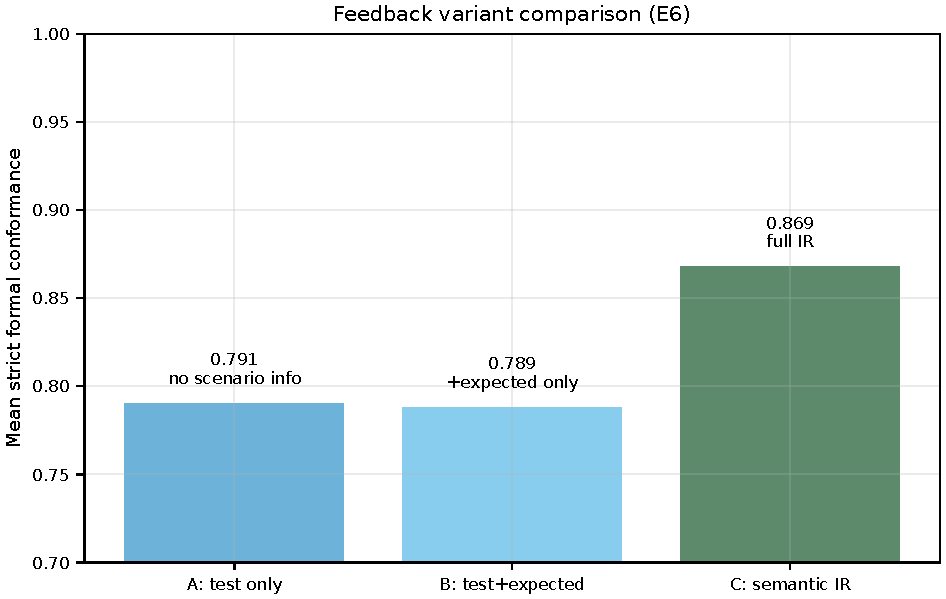
\includegraphics[width=0.95\textwidth]{../hsp-agile/figures/feedback_variant_bar.pdf}
  \caption{E6 feedback variants under full~M ($K{=}3$, $n{=}120$). Variant~C
    (full Semantic IR) +7.7\,pp vs.\ A; CI excludes~0.}
  \label{fig:e6}
\end{figure*}

\begin{table}[t]
\centering
\caption{E6 paired stats, win profile, and equal-$K$ Conf.\ ranking.}
\label{tab:e6}
\footnotesize
\begin{tabular}{lccc}
\toprule
Contrast / mode & W/L/T or $n$ & Conf.\ / $\Delta$ & 95\% CI \\
\midrule
E6 C$-$A & 14/4/102 & $+7.7$\,pp & $[2.3,\,13.6]$ \\
E6 C$-$B & 14/4/102 & $+8.0$\,pp & $[2.2,\,14.0]$ \\
Win profile & 13/14 zero-A & \texttt{others}/arith. & --- \\
Equal-$K$ B2 & 120 & 97.5\% & --- \\
Equal-$K$ \texttt{M\_eq} & 120 & \textbf{100.0\%} (${+}2.5$) & 3/0/117 \\
\bottomrule
\end{tabular}
\end{table}

\begin{table}[t]
\centering
\caption{Defect-class $\leftrightarrow$ evidence map.}
\label{tab:defect-map}
\footnotesize
\begin{tabular}{@{}lll@{}}
\toprule
Defect class & Primary evidence & Supports \\
\midrule
Order / preemption & $\Phi_i$; E2 mutants & dual-gate prevention \\
\texttt{others}/arith.\ rescue & E6 win coding & feedback mechanism \\
Saturated easy tasks & pilots ($n{\ge}28$) & default B2 \\
\bottomrule
\end{tabular}
\end{table}

\subsection{RQ2: Prevention under the dual gate (E2)}
On implementation-screening mutants ($n{=}852$), M reaches PDR 95.0\% / FAR
5.0\% vs.\ B2 91.2\% / 8.8\%; paired bootstrap 95\% CIs on the gaps exclude
zero (Fig.~\ref{fig:prev}).
The absolute PDR lift is ${+}3.8$\,pp on this mutant population.
Fixed-oracle Conf.\ ablations vs.\ strengthened M: removing repair $-$25.8\,pp;
removing formal checker $-$17.5\,pp; removing pattern guard $0.0$\,pp on Conf.\
under an advisory gate.  These ablations isolate conformance effects, whereas
E2 evaluates the bundled dual gate; they do not separately identify the
screen's causal contribution to prevention.

\begin{figure*}[t]
  \centering
  \begin{minipage}{0.48\textwidth}
    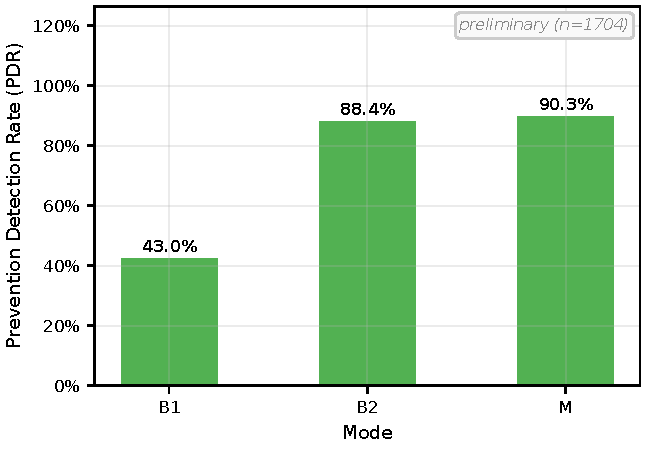
\includegraphics[width=\linewidth]{../hsp-agile/figures/prevention_bar.pdf}
    \caption{E2 aggregate PDR by mode.}
    \label{fig:prev}
  \end{minipage}\hfill
  \begin{minipage}{0.48\textwidth}
    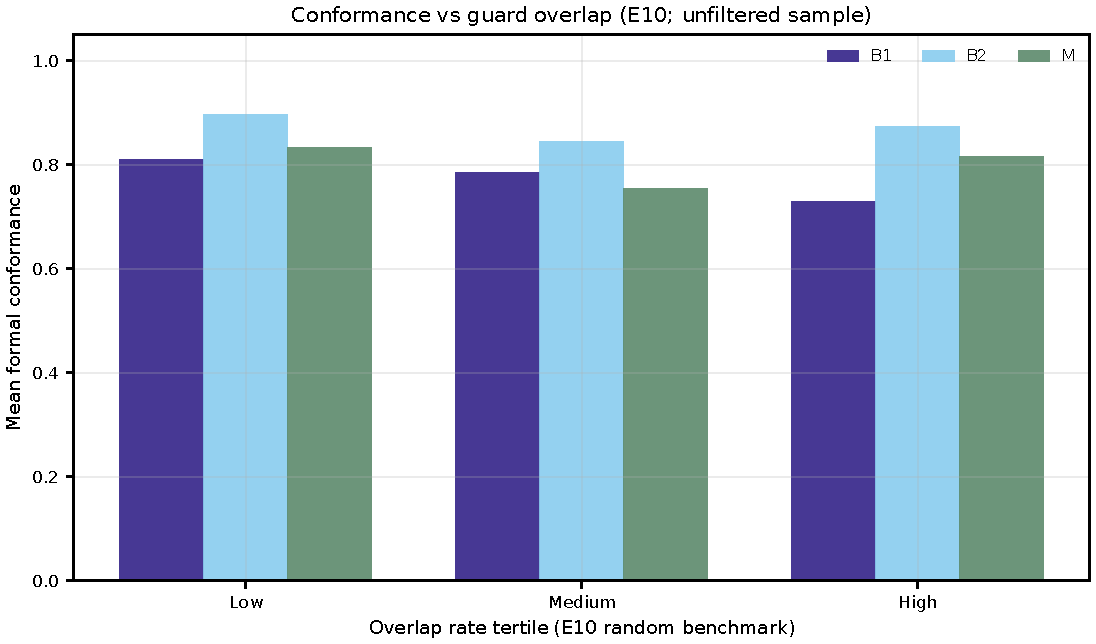
\includegraphics[width=\linewidth]{../hsp-agile/figures/performance_vs_overlap.pdf}
    \caption{E10 Conf.\ vs.\ overlap tertile (non-monotone).}
    \label{fig:overlap}
  \end{minipage}
\end{figure*}

\subsection{RQ3: Cross-model behavior and matched-budget evidence}
The catch-all failure is not specific to one model family, but the benefit of
additional feedback depends on remaining repair headroom.
On \texttt{gemini-2.5-flash}, frozen hard seeds yield ${+}26.5$\,pp for
scenario-aware feedback over test-only feedback (pooled $n{=}80$, CI excludes
zero).  On industrial-pattern tasks, GPT-4o and Claude both reach 100.0\%
with B2 while the fuller mode reaches 95.5\%; DeepSeek retains more headroom
(80.7\% for B2 and 72.5\% for M).  These results show that stronger models can
saturate under ordinary test feedback; they support conditional deployment,
not a universal gain from the full pipeline.

\begin{table}[t]
\centering
\caption{Cross-model industrial-pattern results ($n{=}31$; mean Conf.\ \%).}
\label{tab:cross-model}
\footnotesize
\begin{tabular}{lccc}
\toprule
Model & B1 & B2 & M \\
\midrule
GPT-4o & 95.5 & \textbf{100.0} & 95.5 \\
Claude 4.6 & 95.5 & \textbf{100.0} & 95.5 \\
DeepSeek & 52.7 & \textbf{80.7} & 72.5 \\
\bottomrule
\end{tabular}
\end{table}

Equal-$K$ Conf.\ ranking (Table~\ref{tab:e6}): \texttt{M\_eq} 100.0\% vs.\ B2
97.5\% (${+}2.5$\,pp; 3/0/117)---matched budget, not a substitute for E6.
Unified external equal-$K$: GitHub B2${=}$\texttt{M\_eq} 89.9\%; HKCA09 both
100\%; desensitized both 100\%.
Strengthened E1 ($K{=}5$ bundle, Table~\ref{tab:e1}) sits near ceiling.
E12: B2 reaches 100\% on every seed; M mean 99.7\% across seeds.

\begin{table}[t]
\centering
\caption{E1 near-ceiling ranking (fixed oracle; $K{=}5$ bundle for M).}
\label{tab:e1}
\footnotesize
\begin{tabular}{lccc}
\toprule
Mode & Mean Conf. & Strict & Mean LLM calls \\
\midrule
B1 & 84.2\% & 84.2\% & 1.00 \\
B2 & 98.3\% & 98.3\% & $\sim$1.18 \\
M ($K{=}5$ bundle) & \textbf{100.0\%} & \textbf{100.0\%} & $\sim$1.16 \\
\bottomrule
\end{tabular}
\end{table}

\subsection{RQ4: Deployment boundary and public-corpus transfer}
Canonical E3/E10 tertiles are non-monotone (Fig.~\ref{fig:overlap}): escalate
on Accept/FAR and headroom, not on overlap density alone
(Table~\ref{tab:deploy}).
On fixed-oracle E1, mean LLM calls for B2 ($\sim$1.18) and strengthened M
($\sim$1.16) are comparable; wall-clock means are 9.6\,s (B2) vs.\ 10.5\,s (M).

\begin{table}[t]
\centering
\caption{Deployment boundary: release bar and repair headroom.}
\label{tab:deploy}
\footnotesize
\begin{tabular}{@{}lll@{}}
\toprule
Signal & Prefer B2 & Prefer M \\
\midrule
Default & Mean Conf./latency & --- \\
Release & Mean Conf.\ OK & Accept${=}1$ \\
Prevention & --- & FAR${\le}5\%$ \\
Headroom & Saturated endpoint & Collapsed test-only Conf.\ (E6) \\
Overlap tertile & Non-monotone & Not a trigger \\
\bottomrule
\end{tabular}
\end{table}

\subsubsection{Public and published corpora}
\label{sec:ext}
Desensitized published pilot ($n{=}28$): B1/B2/\texttt{M\_eq} all 100.0\%.
GitHub harvest ($n{=}48$): B2/\texttt{M\_eq} 89.9\% vs.\ B1 85.8\%.
HKCA09$\rightarrow$FSF ($n{=}35$): B1 74.3\% / B2${=}$\texttt{M\_eq} 100\%.
These ranking ties support B2 as the default for mean Conf.
Where one-shot saturates, HKCA09 hard-seed repair (wrong\_relop:
\texttt{semantic\_ir} 82.0\% vs.\ test\_only 69.3\%, ${+}12.7$\,pp; CI may
include~0) is scoped external support.
Provenance: reconstructions / public harvest---not proprietary dumps.

\begin{table}[t]
\centering
\caption{External corpora (mean Conf.\ \%).}
\label{tab:ext}
\footnotesize
\begin{tabular}{lccc}
\toprule
Corpus & B1 & B2 & M / \texttt{M\_eq} \\
\midrule
Industrial-pattern ($n{=}31$, gpt-4o) & 95.5 & \textbf{100.0} & 95.5 \\
Desens.\ published ($n{=}28$) & 100.0 & \textbf{100.0} & \textbf{100.0} \\
GitHub harvest ($n{=}48$) & 85.8 & \textbf{89.9} & \textbf{89.9} \\
HKCA09 FSF ($n{=}35$) & 74.3 & \textbf{100.0} & \textbf{100.0} \\
Equal-$K$ BENCH-120 & --- & 97.5 & \textbf{100.0} \\
\bottomrule
\end{tabular}
\end{table}

\subsubsection{Public ACL interception case}
The aggregate results are complemented by
\texttt{enforce\_api\_acl}, an ordered API-access contract reconstructed from
the public RealSpec/harvest family.  The contract denies guests, requires
step-up MFA for high scope, permits narrow admin/reader bands, and fails closed
on \texttt{OTHERWISE}.  An LLM-shaped candidate passes the busy guest-deny and
admin-permit tests but contains two residual defects: high scope without MFA
is permitted, and the catch-all branch fails open.  A first-match witness
$(\mathit{role}{=}2,\mathit{scope}{=}2,\mathit{mfa}{=}1)$ forces the residual
branch; the candidate returns permit, so Conf${<}1$ and the dual-gate check
refuses release.  This reproducible case illustrates the operational target
of the method, while remaining smaller than a repository-scale industrial
study.

\subsubsection{Scope of transfer}
The controlled causal estimate remains E6 on the primary endpoint; Gemini
supports the repair mechanism on frozen hard seeds, while GPT-4o and Claude
demonstrate saturation on industrial-pattern tasks.  Public and reconstructed
corpora support the deployment boundary, but they do not constitute
repository-scale validation.

%======================================================================
\section{Discussion}
%======================================================================
\runin{Practice.}
Match feedback depth to the release bar: B2 for mean Conf.\ / latency; M when
dual-gate Accept or FAR${\le}5\%$ is required \emph{and} repair headroom
remains (E6 rescue when test-only Conf.\ collapses).
External pilots reinforce default B2 on mean Conf.
A practical playbook: (i)~B2 inner loop; (ii)~pre-release M with Accept;
(iii)~track FAR on a frozen mutant pack; (iv)~escalate if FAR drifts or Accept
failures cluster.

\runin{Limitations.}
BENCH-120 is synthetic and overlap-filtered; E10 and public pilots probe, but
do not bound, transfer.
Finite witnesses approximate Conf.; the others-witness measurement correction
previously inflated false failures.
LLM non-determinism is mitigated by $T_\text{repair}{=}0$ and paired tests;
the $K{=}5$ E1 bundle combines several mechanisms and is used only as
near-ceiling context.
Published reconstructions and harvests are not production dumps; vendor NDA
\texttt{.asfl} pilots remain future work.  The screen catalogue and mutation
operators are author-selected from SOFL fault patterns; E2 therefore estimates
rejection on that constructed first-order distribution, not completeness or
repository-wide safety.
Ceiling effects on stronger models shrink E6 deltas---report headroom when
transferring claims.
E14 shows that length-matched execution traces can outperform the tested
scenario-aware record on mean Conf.; E6 therefore establishes improvement
over unstructured test feedback rather than superiority over every structured
feedback design.
B2 leads every E12 seed (100\%); M mean is 99.7\% across seeds.

\runin{Reproducibility.}
Authoritative numbers and run ids ship with the artefact package
(\texttt{AUTHORITATIVE\_NUMBERS.md}, benchmark JSON, summarisation scripts).
Primary claims cite those run directories rather than ad-hoc aggregates.

%======================================================================
\section{Conclusion}
%======================================================================
HSP-Agile pairs first-match witnesses, scenario-aware repair feedback, and a
dual-gate acceptance check for ordered-guard specifications.
The central result is a bounded acceptance check: release only under
$\mathrm{Accept}\Leftrightarrow\mathrm{Conf}{=}1\wedge\mathrm{Screen}{=}\mathit{pass}$.
Under headroom, E6 yields ${+}7.7$\,pp vs.\ test-only at $K{=}3$ (CI
excludes~0; 14/14 catch-all rescues).
E2 supports the gate on the evaluated mutant population at FAR 5.0\% vs.\
8.8\%.
Deploy B2 by default; escalate for Accept or FAR${\le}5\%$ with headroom.
Future work includes NDA vendor \texttt{.asfl} pilots, adaptive~$K$, and
SpecIR adapters beyond SOFL/FSF.

\bibliographystyle{IEEEtran}
\bibliography{../hsp-agile/bib/references}
\balance
\end{document}
